\documentclass[../main.tex]{subfiles}
\graphicspath{{figures/}{../figures/}}

\begin{document}
% \todo[color=green!40]{完成问题三模型的求解(sections/q3\_solution)}

调整导弹的飞行速度,利用问题4的模型对三架无人机的投弹策略重新进行优化。同理使用遗传算法,利用Python求解,结果见图\ref{Figure_1}。
\begin{figure}[H]
\centering
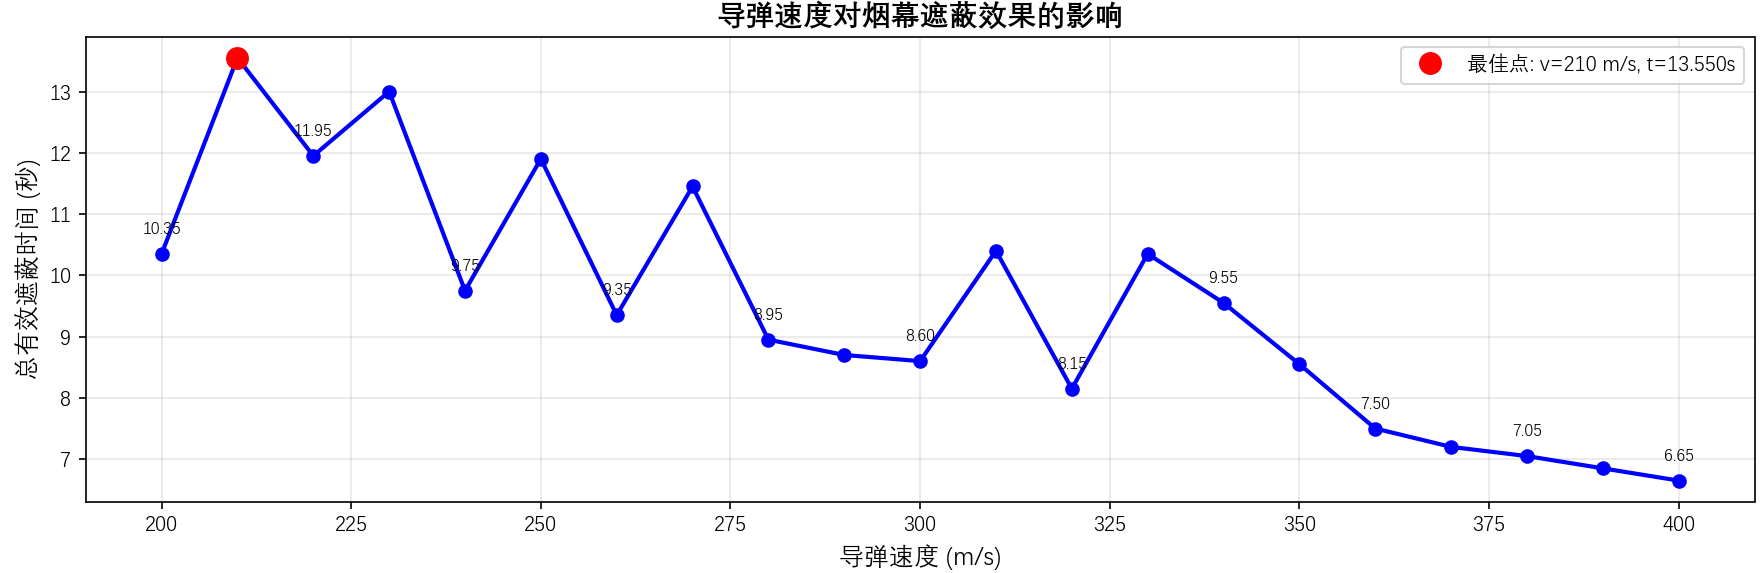
\includegraphics[scale=0.35]{灵敏度分析图.png}
\caption{导弹速度与有效时间关系}
\label{Figure_1}
\end{figure}
由图\ref{Figure_1}可知\textbf{有效时间对导弹的飞行速度的变化是敏感的},并且随着导弹速度增加有效时间逐渐减小。





\end{document}